\begin{table}[htbp]
	\centering
	\scriptsize
	\subtable[Pattern Recognition Example: Memory Time Domain]{%
		\begin{tabular}{l | ccccc} % creating eight columns
	  	\hline
		Triple  & \multicolumn{5}{c}{Slots}  \\
		in & \multicolumn{5}{c}{Number}  \\
		Window  & 1 & 10 & 100 & 1000&10000\\
		\hline
			\hline
		1	   &\begin{minipage}{.085\textwidth}\vspace{2pt}     							
     			 	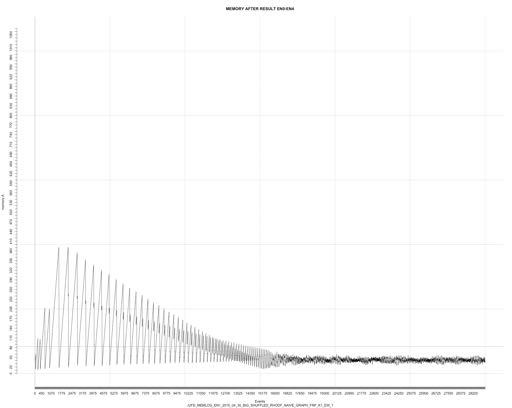
\includegraphics[width=\linewidth]{images/mema-graph/N1}
    				 \end{minipage}\\			
		10	   & \begin{minipage}{.085\textwidth}\vspace{2pt}     							
     			 	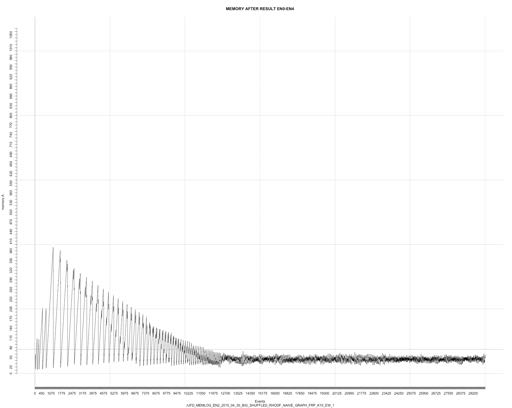
\includegraphics[width=\linewidth]{images/mema-graph/N2}
    				\end{minipage}
    			   & \begin{minipage}{.085\textwidth}\vspace{2pt}     							
     			 	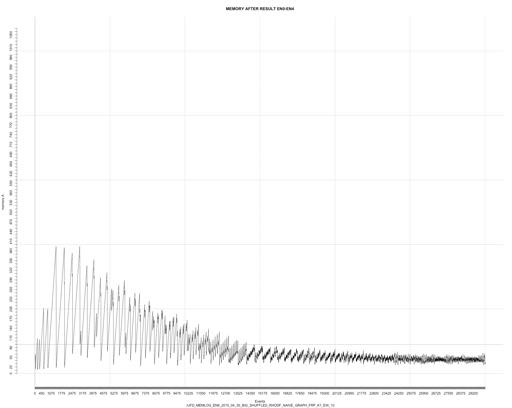
\includegraphics[width=\linewidth]{images/mema-graph/N6}
    				 \end{minipage}\\		
		100	   & \begin{minipage}{.085\textwidth}\vspace{2pt}     							
     			 	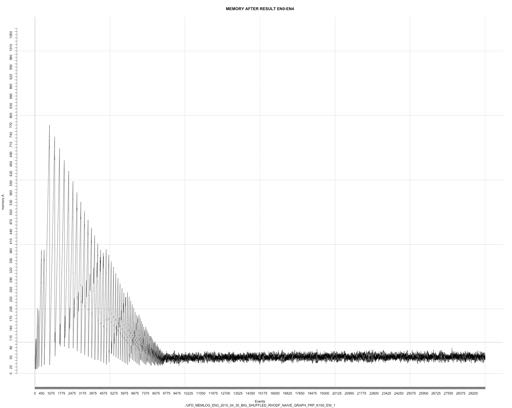
\includegraphics[width=\linewidth]{images/mema-graph/N3}
    				 \end{minipage}
    			   & \begin{minipage}{.085\textwidth}\vspace{2pt}     							
     			 	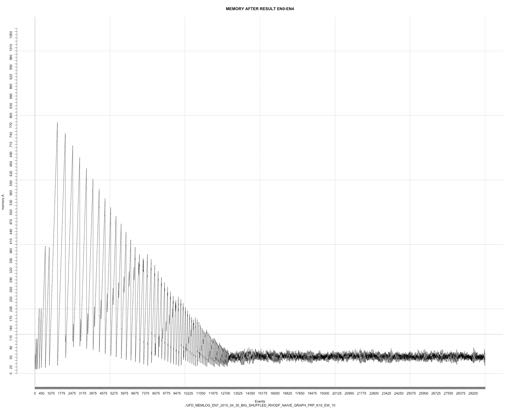
\includegraphics[width=\linewidth]{images/mema-graph/N7}
    				 \end{minipage}
    			   &	 \begin{minipage}{.085\textwidth}\vspace{2pt}     							
     			 	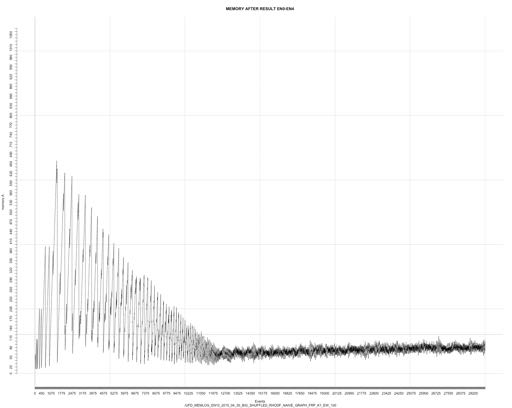
\includegraphics[width=\linewidth]{images/mema-graph/N10}
    				 \end{minipage}\\	
		1000   &	 \begin{minipage}{.085\textwidth}\vspace{2pt}     							
     			 	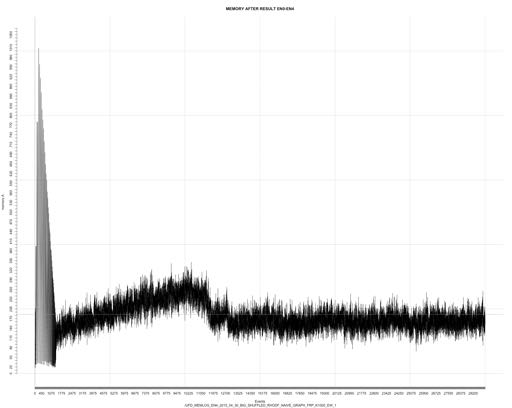
\includegraphics[width=\linewidth]{images/mema-graph/N4}
    				 \end{minipage}
    			   &	 \begin{minipage}{.085\textwidth}\vspace{2pt}     							
     			 	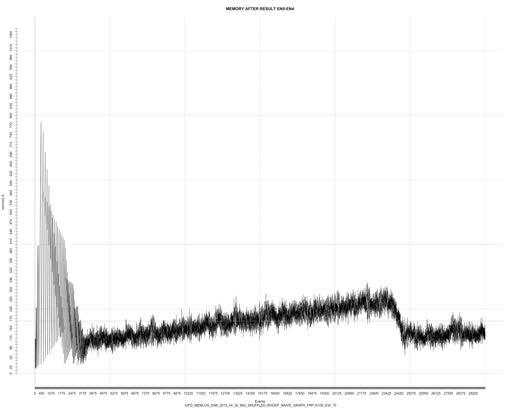
\includegraphics[width=\linewidth]{images/mema-graph/N8}
    				 \end{minipage}
    			   &	 \begin{minipage}{.085\textwidth}\vspace{2pt}     							
     			 	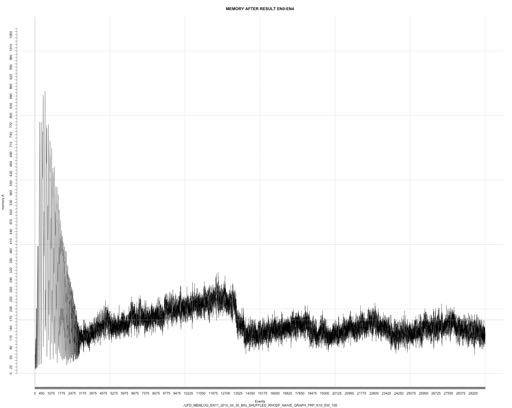
\includegraphics[width=\linewidth]{images/mema-graph/N11}
    				 \end{minipage}
    			   &	 \begin{minipage}{.085\textwidth}\vspace{2pt}     							
     			 	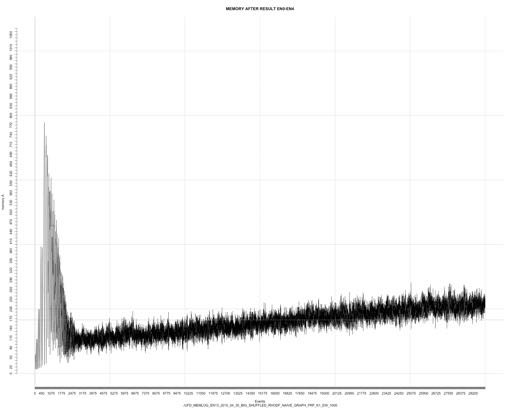
\includegraphics[width=\linewidth]{images/mema-graph/N13}
    				 \end{minipage}\\
		10000  &	 \begin{minipage}{.085\textwidth}\vspace{2pt}     							
     			 	
\includegraphics[width=\linewidth]{images/mema-graph/N5}
    				 \end{minipage}
    			   &	 \begin{minipage}{.085\textwidth}\vspace{2pt}     							
     			 	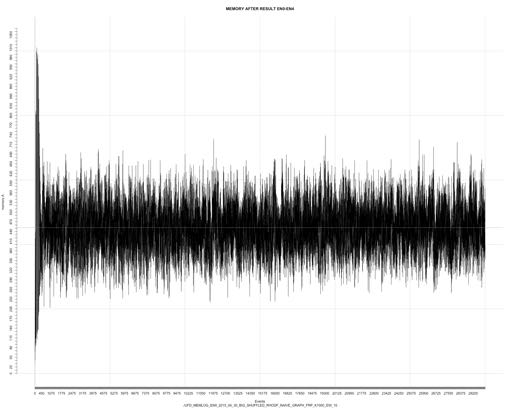
\includegraphics[width=\linewidth]{images/mema-graph/N9}
    				 \end{minipage}
    			   &	 \begin{minipage}{.085\textwidth}\vspace{2pt}     							
     			 	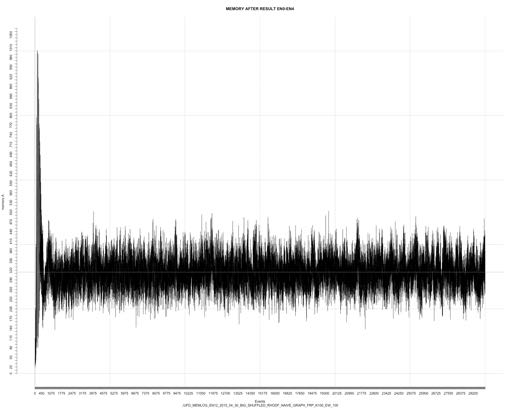
\includegraphics[width=\linewidth]{images/mema-graph/N12}
    				 \end{minipage}
    			   &	 \begin{minipage}{.085\textwidth}\vspace{2pt}     							
     			 	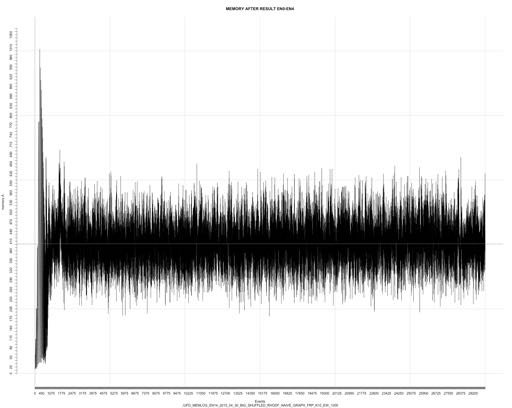
\includegraphics[width=\linewidth]{images/mema-graph/N14}
    				 \end{minipage}
    			   &	 \begin{minipage}{.085\textwidth}\vspace{2pt}     							
     			 	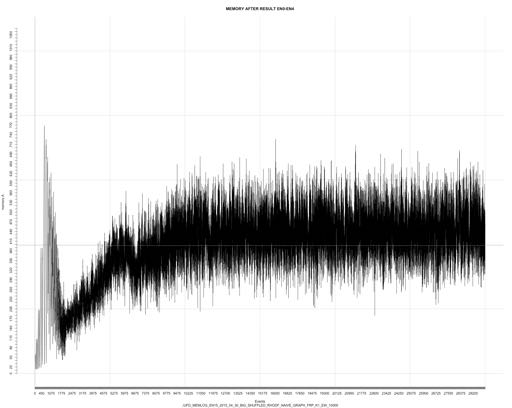
\includegraphics[width=\linewidth]{images/mema-graph/N15}
    				 \end{minipage}\\
		\hline % inserts single-line
	 \end{tabular}
	}
	\subtable[Pattern Recognition Example: Memory Distribution]{%
		\begin{tabular}{l | ccccc} % creating eight columns
	  	\hline
		Triple  & \multicolumn{5}{c}{Slots}  \\
		in & \multicolumn{5}{c}{Number}  \\
		Window  & 1 & 10 & 100 & 1000&10000\\
		\hline
			\hline
		1	   &\begin{minipage}{.085\textwidth}\vspace{2pt}     							
     			 	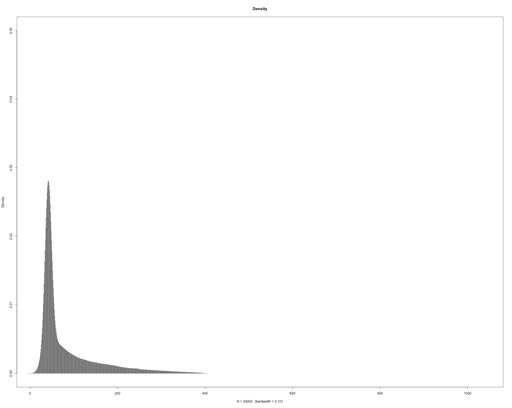
\includegraphics[width=\linewidth]{images/mema-dens-graph/N1}
    				 \end{minipage}\\			
		10	   & \begin{minipage}{.085\textwidth}\vspace{2pt}     							
     			 	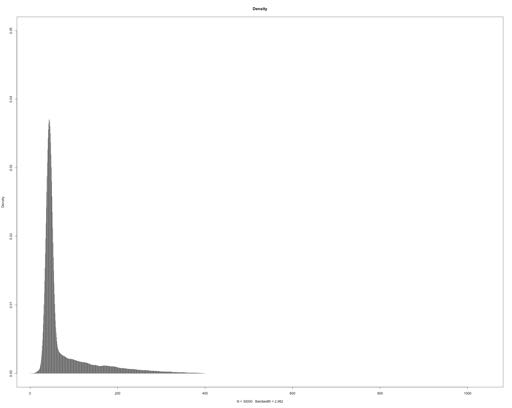
\includegraphics[width=\linewidth]{images/mema-dens-graph/N2}
    				\end{minipage}
    			   & \begin{minipage}{.085\textwidth}\vspace{2pt}     							
     			 	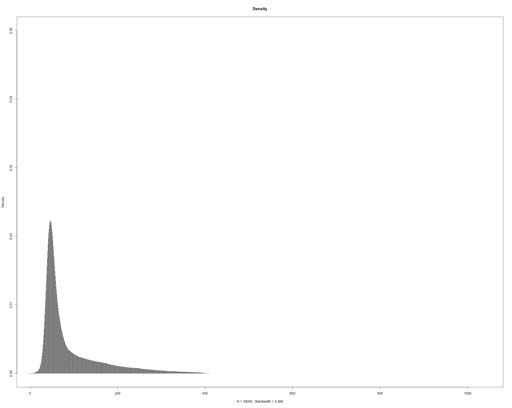
\includegraphics[width=\linewidth]{images/mema-dens-graph/N6}
    				 \end{minipage}\\		
		100	   & \begin{minipage}{.085\textwidth}\vspace{2pt}     							
     			 	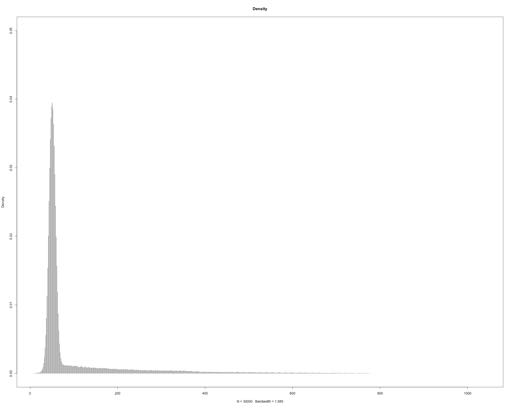
\includegraphics[width=\linewidth]{images/mema-dens-graph/N3}
    				 \end{minipage}
    			   & \begin{minipage}{.085\textwidth}\vspace{2pt}     							
     			 	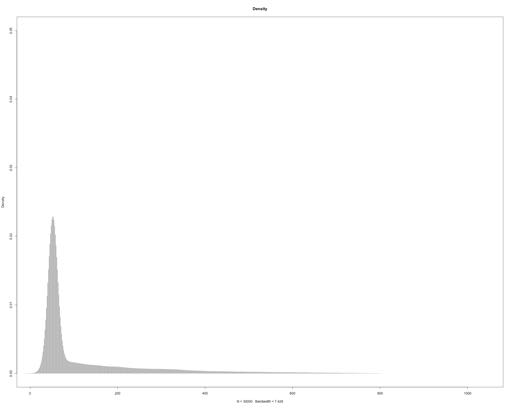
\includegraphics[width=\linewidth]{images/mema-dens-graph/N7}
    				 \end{minipage}
    			   &	 \begin{minipage}{.085\textwidth}\vspace{2pt}     							
     			 	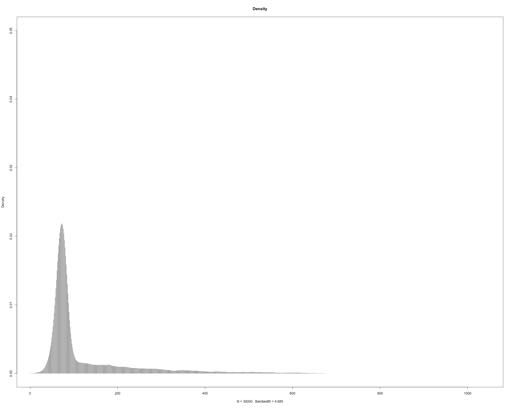
\includegraphics[width=\linewidth]{images/mema-dens-graph/N10}
    				 \end{minipage}\\	
		1000   &	 \begin{minipage}{.085\textwidth}\vspace{2pt}     							
     			 	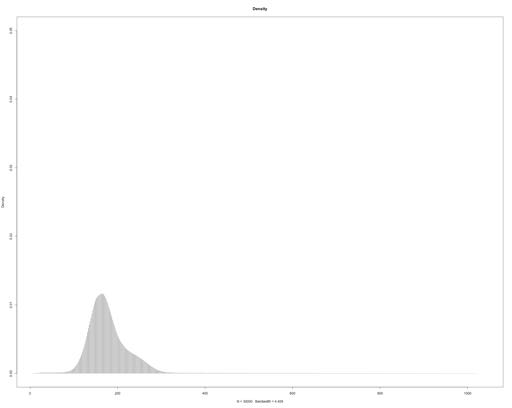
\includegraphics[width=\linewidth]{images/mema-dens-graph/N4}
    				 \end{minipage}
    			   &	 \begin{minipage}{.085\textwidth}\vspace{2pt}     							
     			 	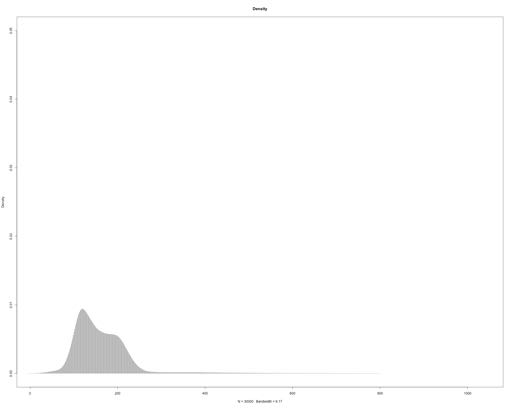
\includegraphics[width=\linewidth]{images/mema-dens-graph/N8}
    				 \end{minipage}
    			   &	 \begin{minipage}{.085\textwidth}\vspace{2pt}     							
     			 	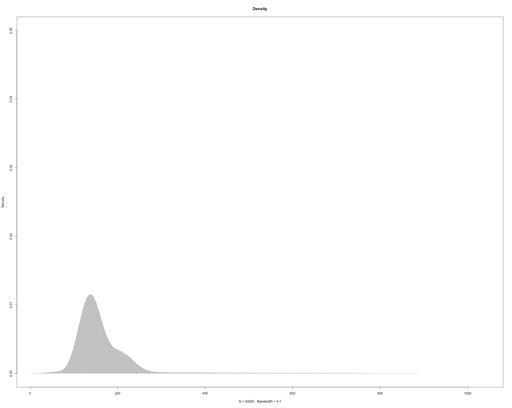
\includegraphics[width=\linewidth]{images/mema-dens-graph/N11}
    				 \end{minipage}
    			   &	 \begin{minipage}{.085\textwidth}\vspace{2pt}     							
     			 	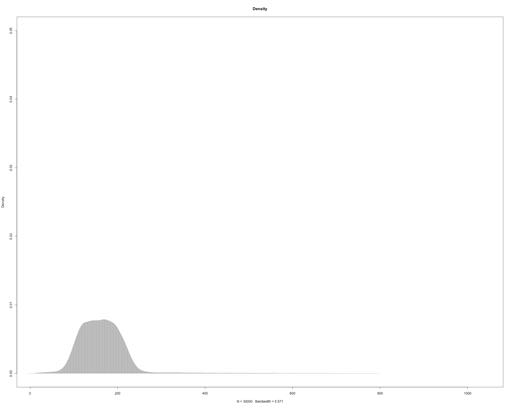
\includegraphics[width=\linewidth]{images/mema-dens-graph/N13}
    				 \end{minipage}\\
		10000  &	 \begin{minipage}{.085\textwidth}\vspace{2pt}     							
     			 	
\includegraphics[width=\linewidth]{images/mema-dens-graph/N5}
    				 \end{minipage}
    			   &	 \begin{minipage}{.085\textwidth}\vspace{2pt}     							
     			 	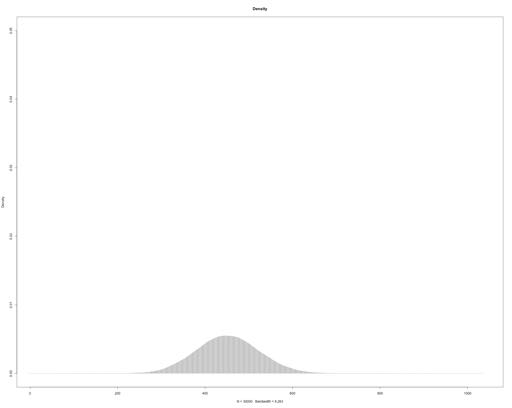
\includegraphics[width=\linewidth]{images/mema-dens-graph/N9}
    				 \end{minipage}
    			   &	 \begin{minipage}{.085\textwidth}\vspace{2pt}     							
     			 	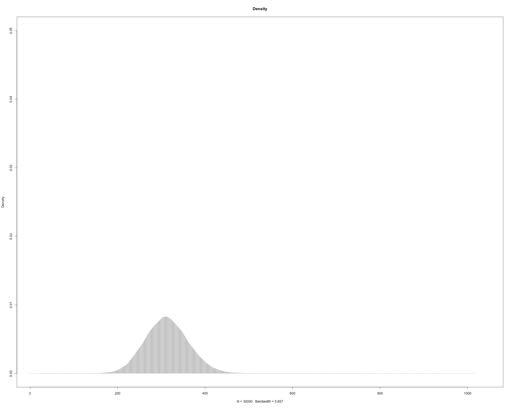
\includegraphics[width=\linewidth]{images/mema-dens-graph/N12}
    				 \end{minipage}
    			   &	 \begin{minipage}{.085\textwidth}\vspace{2pt}     							
     			 	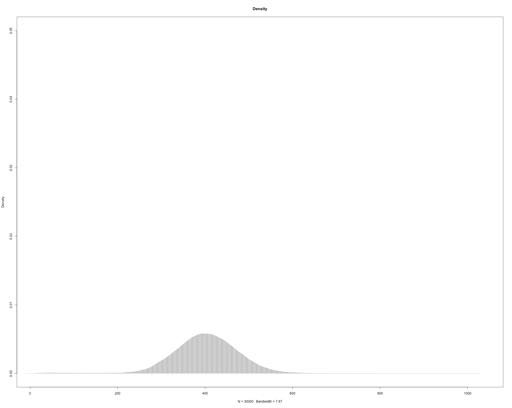
\includegraphics[width=\linewidth]{images/mema-dens-graph/N14}
    				 \end{minipage}
    			   &	 \begin{minipage}{.085\textwidth}\vspace{2pt}     							
     			 	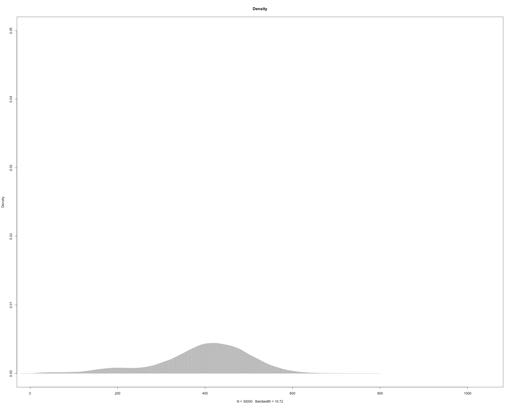
\includegraphics[width=\linewidth]{images/mema-dens-graph/N15}
    				 \end{minipage}\\
		\hline % inserts single-line
	 \end{tabular}
	}
	\caption[\textsc{Analyser} Investigation Stack - Level 2 - Pattern Recognition Examples]{Two examples of pattern recognition. Level 2 exploits  easy-to-read layouts which highlights the experiment difference to enable \textit{Inter Experiment} comparisons.} 
	\label{tab:pattern-examples}	
\end{table}